\documentclass[conference]{IEEEtran}
\IEEEoverridecommandlockouts
% The preceding line is only needed to identify funding in the first footnote. If that is unneeded, please comment it out.
\usepackage{cite}
\usepackage{amsmath,amssymb,amsfonts}
\usepackage{algorithmic}
\usepackage{graphicx}
\usepackage{textcomp}
\usepackage{subfigure, booktabs, enumerate, url}
\def\BibTeX{{\rm B\kern-.05em{\sc i\kern-.025em b}\kern-.08em
    T\kern-.1667em\lower.7ex\hbox{E}\kern-.125emX}}
\begin{document}

\title{Bottle Detection in the Wild Using Low-Altitude Unmanned Aerial Vehicles
%\thanks{Identify applicable funding agency here. If none, delete this.}
}
\author{\IEEEauthorblockN{Jinwang Wang, Wei Guo, Ting Pan, Huai Yu, Lin Duan, Wen Yang}
	\IEEEauthorblockA{\textit{School of Electronic Information, Wuhan University} Wuhan, China \\
		\{jwwangchn, weige, ting.pan, yuhuai, duanlin, yangwen\}@whu.edu.cn}

%\author{\IEEEauthorblockN{1\textsuperscript{st} Jinwang Wang}
%\IEEEauthorblockA{\textit{School of Electronic Information, Wuhan University}\\
%Wuhan, China \\
%jwwangchn@whu.edu.cn}
%\and
%\IEEEauthorblockN{2\textsuperscript{nd} Given Name Surname}
%\IEEEauthorblockA{\textit{School of Electronic Information, Wuhan University} \\
%Wuhan, China \\
%email address}
%\and
%\IEEEauthorblockN{3\textsuperscript{nd} Given Name Surname}
%\IEEEauthorblockA{\textit{School of Electronic Information, Wuhan University} \\
%	Wuhan, China \\
%	email address}

}

\maketitle

\begin{abstract}
    
    This paper proposed a vision based bottle detection system for UAV imagery. From UAV's perspective, bottles have huge variation in scale, ratios orientation and shape. Different from the traditional annotation methods using the horizontal bounding box, we use the oriented bounding box to annotate the objects, which is easier to separate the objects from background. It is worth mentioning that we have collected \boldmath $ 25,407 $ UAV images of bottles with size of \boldmath $ 342\times 342 $ pixels in different scenes. 
%These bottles are in a wide variety of scales, ratios, orientations and shapes. 
And we also have annotated these images using oriented bounding box. These fully annotated images contain  \boldmath $ 34,791 $ instances, each of which is annotated by an arbitrary quadrilateral  \boldmath $\{c_x, c_y, h, w, \theta \}$. To build a baseline for bottle detection, we evaluate some state-of-the-art object detection algorithms like  Faster R-CNN, SSD, YOLOv2 and RRPN on our UAV-Bottle Dataset (UAV-BD). Experiments demonstrate that our dataset contributes greatly to the environmental protection applications and are quite challenging due to the difficulties of locating the multi-angle bottles and separating them effectively from the background.
    
   
    % 问题: 近些年来, 无人机被广泛用于遥感应用, 其中一个用途是用于旅游景区丢弃的瓶子的检测, 


\end{abstract}

\begin{IEEEkeywords}
	Bottle Detection, Oriented Bounding Box, UAV-Bottle Dataset
\end{IEEEkeywords}

\section{Introduction}

%0. Abstract
%	1. 建立了一个 UAV-BD 的数据集
%	2. 比较 Faster RCNN, SSD, RRPN, DRBox 算法
%
%1. Introduction
%	1. 建立这个数据集的动机(目的) -> 旅游景区垃圾丛生, 传统人力回收的方式过于危险, 可以使用无人机辅助定位并捡垃圾, 减少工人危险系数 -> 为了实现无人机定位瓶子, 需要检测瓶子 -> 引出数据集
%	
%	2. 无人机的发展, 无人机的特性, 对数据集的影响 -> 引出无人机视角下, 目标的外形与 PASCAL VOC, COCO 等数据集完全不同, 不能使用当前公开的数据集训练模型 (数据的重要性) -> 引出无人机视角下瓶子的特性
%	
%	3. 无人机视角下瓶子的特性 -> (1) 尺寸小, (2) 尺度变化大, (3) 种类多, (4) 具有旋转性, (5) 透明特性, (6) 背景复杂 -> 引出我们建立了 UAV-Bottle Dataset (UAV-DB) 数据集 -> 数据集展示 (一张大图, 下面三张小图)
%	
%	4. 目标检测算法的发展 -> 简要概括传统目标检测算法, 主要是 RCNN, Faster RCNN, Faster RCNN 线和 YOLO SSD 线 -> 发现瓶子旋转特性对模型影响很大, 引出 RRPN 和 DRBox 
%	
%2. UAV-Bottle Dataset
%	1. 无人机视角下数据集特性分析 -> 引出数据集收集和构建方式的合理性 -> (1) 尺寸小(裁剪成小图, 使用具有多尺度特性的算法作为 pipline), (2) 尺度变化大(无人机在不同飞行高度下采集图像, 10m-50m), (3) 种类多(使用尽量多种类的饮料瓶), (4) 具有旋转性(旋转标注, 介绍优点, 并指出传统标注方式的缺点(图示), 使用能使用 RBox 作为 pipline), (5) 透明特性, 训练难度大(选择透明性较好的瓶子), (6) 背景复杂(选择可能出现的场景收集数据, 分为8个场景, 并分类存储, 方便算法针对特定场景进行优化, 展示不同场景下的图像) -> 引出收集方式
%	
%	2. 收集方式 -> 两阶段收集, 无人机飞行高度, 瓶子种类, 背景分类 (展示不同背景下的瓶子), 裁剪方式, 图片大小, 如何处理边界图像
%	
%	3. 数量统计 -> 分场景统计 (1) 大图数量 (2) 小图数量 (3) 大图中目标数量 (4) 小图中目标数量 (5) Scale Angle Ratio 分布特性 (6) train val test 如何划分 (1-4表格展示, 5直方图展示)
%	4. 标注方式 -> 使用旋转框进行标注, 用于训练 RRPN 和 DRBox 等能使用旋转框训练的算法, 对旋转框做最小外接矩形变成传统框(图示), 用于训练传统算法
%
%3. Pipline Experiments and Result
%	1. 使用本数据集训练了四种基于深度学习的算法 Faster RCNN, SSD, RRPN, DRBox
%	2. Faster RCNN 和 SSD 使用原版参数
%	3. 简要介绍 RRPN 和 DRBox 在 Faster RCNN 和 SSD 算法上的改进, 他们如何使用旋转标注框 (画出pipline)
%	4. 针对 UAV-BD 对 RRPN 和 DRBox 的改进 -> (1) 根据 UAB-BD 的数据分布修改了 RRPN 的 Rotation Anchor, (2) 根据 UAV-BD 的数据分布修改了 DRBox 的 prior box
%	5. 对比四种深度学习算法的 PR 曲线和 AP 性能, 给出简要结论 -> 旋转bbox能提高算法的性能
%
%
%4. Conclusion
%	1. 我们建立了 UAV-BD 数据集, 并将公开这个数据集
%	
%	2. 我们使用本数据集训练了 Faster RCNN, SSD, RRPN, DRBox, 并比较了他们之间的性能差异, 得出旋转标注对模型训练具有一定优势
%
%5. Reference


\label{sec:intro}

%% 1. 建立本数据集的动机和目的

Nowadays, with the popularity of tourist attractions, there is a lot of rubbish, especially bottles, need to recycle. However, these bottles are mainly collected by human observation, which is time-consuming, laborious and dangerous. In order to solve these problems, we use the unmanned aerial vehicle (UAV) to locate and even recycle bottles. We also build a UAV bottle dataset (UAV-BD) to locate bottles more effectively.


%% 2. UAV 的发展, 拍摄图像的特性, 对目标检测的影响 -> 引出无人机视角下瓶子的特性

Detecting objects in UAV images plays an important role in many applications and has received significant attention in recent years\cite{UAV2}. However, it is still a challenging problem due to the high resolution with the extremely high level of detail, various shooting platform, limited annotated data, and limited processing time for real-time applications\cite{car_detection}. In UAV images, the bottle looks completely different from the bottle in datasets such as PASCAL VOC\cite{PASCALVOC}, Microsoft COCO\cite{COCO}, etc. The difference between PASCAL VOC and our dataset is shown in Fig.\ref{bottle_VOC_UAV}.

\begin{figure}
	\centering
	\subfigure[Bottles in PASCAL VOC]
	{
		\label{bottle_VOC}
		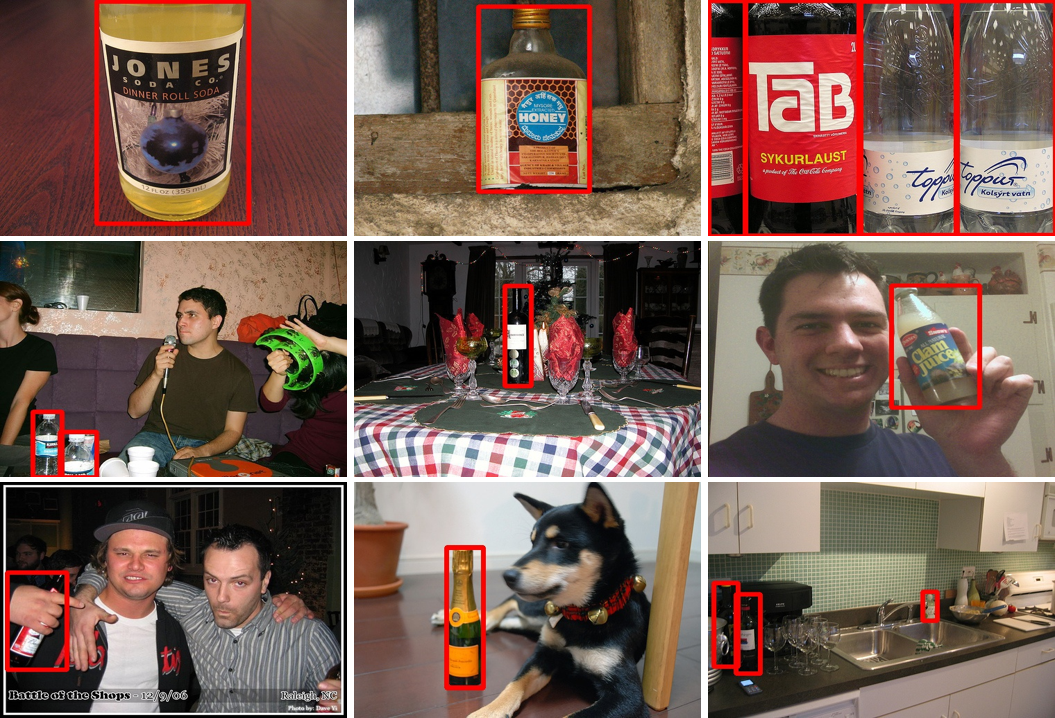
\includegraphics[height=0.37\linewidth]{images/bottle_VOC.png}
	}
	\subfigure[Bottles in UAV images]
	{
		\label{bottle_UAV}
		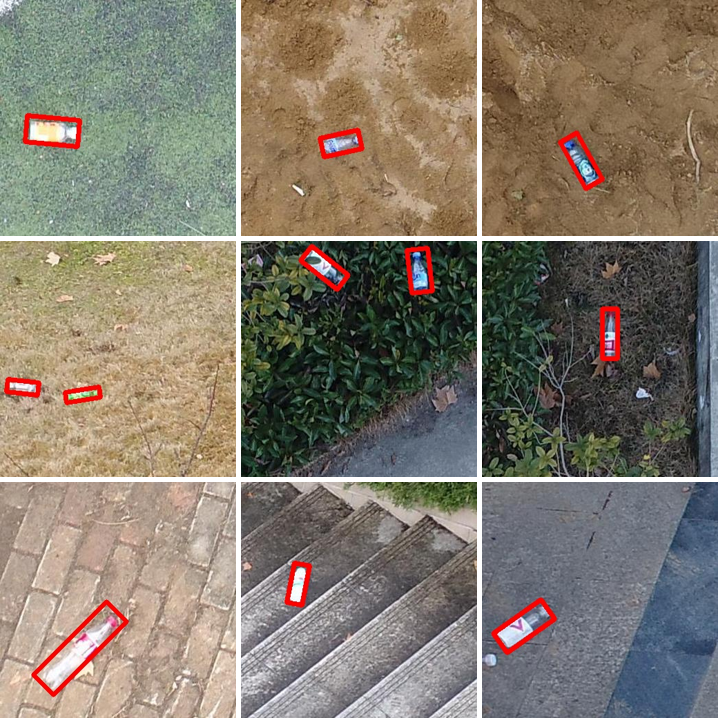
\includegraphics[height=0.37\linewidth]{images/bottle_UAV.png}
	}
	
	\caption{Comparison of bottles in PASCAL VOC dataset and UAV images}
	\label{bottle_VOC_UAV}
\end{figure}

%% 3. 无人机视角下瓶子的特性

As to UAV images, detecting bottles exists several unique challenges. First, the size of bottles is very small, which is generally less than $ 50\times 50 $ pixels. At the same time, due to the different altitudes of the UAV system, the size of bottles differs in scale. Second, in UAV images, the backgrounds of the bottles are very complex which results in poor performance of the general algorithm. Third, in contrast to conventional object detection datasets, where objects are generally oriented upward due to gravity\cite{DOTA}, the bottles in UAV images often appear with arbitrary orientations depending on the shooting angle of the UAV camera, as illustrated in Fig.\ref{bottle_UAV}. Fourth, the plastic bottles are transparent, so the background will can be seen through the bottle, increasing the difficulty of detection. In order to abtain the better performance of an algorithm for the bottle detection problem, we establish a large scale bottle detection dataset and benchmark using UAV, which we call UAV-Bottle Dataset (UAV-BD).

%% 4. 目标检测算法的发展
%% 4.1 深度学习的算法
%% 4.2 基于旋转框的目标检测算法
%Object detection is one of the most challenging tasks in computer vision and has attracted a lot of attention all the time\cite{DRBox}. 
As the development of deep learning, convolutional neural networks(CNN) has been applied to solve the object detection problem and the methods based on CNN have achieved state-of-the-art performance\cite{DRBox}. Most of the existing detection methods use the horizonal bounding boxes to locate objects in images. The horizonal bounding box is a rotation variant data structure, but it works badly when the detector deals with orientation variations of target objects. To make the approach insensitive to objects in-plane rotation, some efforts are made either adjusting the orientation or trying to extract rotation insensitive features. Unlike these methods which try to eliminate the effect of rotation on the feature level, we prefer to make the rotation information useful for feature extraction so that the detection results involve the angle information. Therefore, the detection results are rotatable, whereas the performance of the detector is rotation invariant\cite{DRBox}.

\section{UAV-Bottle Dataset}
\label{sec:dataset}


%% 1. 图片收集方式
\subsection{Dataset collection}
\label{ssec:image_collection}

In the introduction section, we analyzed the challenges that bottle detection may encounter in the UAV perspective.
\begin{itemize}
	%% 1. 尺度问题
	\item The size of the bottles is very small and their scales change very much in UAV images. For solving this problem, we collect images at different flight altitudes of the UAV.
	
	%% 2. 背景复杂
	\item In UAV images, the backgrounds of the bottles are very complex. In order to increase the diversity of dataset, we classify the possible scenes and divide them into eight scenes, each with a different number of images. Eight scenes are illustrated in Fig.\ref{fig:dataset-original-image} and Fig.\ref{fig:dataset-cut-image}. In Fig.\ref{fig:dataset-original-image}, we show eight full images of eight scenes whose sizes are $ 5472\times 3078 $. In Fig.\ref{fig:dataset-cut-image}, we show the segmented images of eight scenes, each scene contains three images whose size are $ 342 \times 342 $.
	
	%% 3. 瓶子旋转
	\item The bottles in UAV images often appear with arbitrary orientations. We find the orientation of bottles will affect the robustness of the trained model, so we annotated images by using the oriented bounding box.
	
	%% 4. 瓶子透明
	\item The plastic bottles as rubbish are usually transparent, so the background can be seen from the bottle, increasing the difficulty of detection. Our dataset includes a lot of transparent bottles, so we can use this large dataset to train a robust model.
\end{itemize}
%\begin{enumerate}[1. ]
%	%% 1. 尺度问题
%	\item The size of the bottles is very small, their sizes are generally less than $ 50\times 50 $ pixels. At the same time, due to the different altitudes of the UAV, their scales change very much. For solving this problem, we collect images at different flight altitudes of the UAV.
%	
%	%% 2. 背景复杂
%	\item In UAV images, the backgrounds of the bottles are very complex, resulting in poor performance of the general algorithm. In order to increase the diversity of dataset, we classify the possible scenes and divide them into eight scenes, each with a different number of images. Eight scenes are illustrated in Fig.\ref{fig:dataset-original-image} and Fig.\ref{fig:dataset-cut-image}. In Fig.\ref{fig:dataset-original-image}, we show eight full images of eight scenes whose sizes are $ 5472\times 3078 $. In Fig.\ref{fig:dataset-cut-image}, we show the segmented images of eight scenes, each scene contains three images whose size are $ 342 \times 342 $.
%	
%	%% 3. 瓶子旋转
%	\item In contrast to conventional object detection datasets, the bottles in UAV images often appear with arbitrary orientations, depending on the perspective of the UAV camera. We find the orientation of bottles will affect the robustness of the trained model, so we annotated images by using the oriented bounding box.
%	
%	%% 4. 瓶子透明
%	\item The plastic bottles as rubbish are usually transparent, so the background can be seen from the bottle, increasing the difficulty of detection. Our dataset includes a lot of transparent bottles, so we can use this large dataset to train a robust model.
%\end{enumerate}



The UAV platform used in this work is a DJI Phantom 4 quadcopter integrated with a 3-axis stabilized gimbal.

Images are collected by a camera mounted on UAV. The resolution of the full images are $ 5472\times 3078 $. For dataset collection, we followed the following three key suggestions: (1) collecting images with bottles of a wide range of scale and aspect ratios; (2) collecting images with bottles of different background scenes; (3) collecting images with bottles of different orientations; (4) using as many types of bottles as possible. 


To collect images covering bottles of a wide range of scales and aspect ratios, images at different flight altitudes of UAV, ranging from $ 10m $ to $ 30m $ are collected. Eight background scenes are chosen and annotated in our UAV-BD, including \textit{Bush forest land}, \textit{Waste land}, \textit{Step}, \textit{Forest land}, \textit{Flat ground}, \textit{Plastic stadium}, \textit{Sand land} and \textit{Grassland}. In this work, UAV images were collected from two periods. For each period, images are collected by using different bottles and different flight altitudes. Totally, images two periods are collected for establishing the dataset. The background scenes are selected according to whether a kind of scene is common and its value for real-world applications\cite{DOTA}.

\begin{figure}
	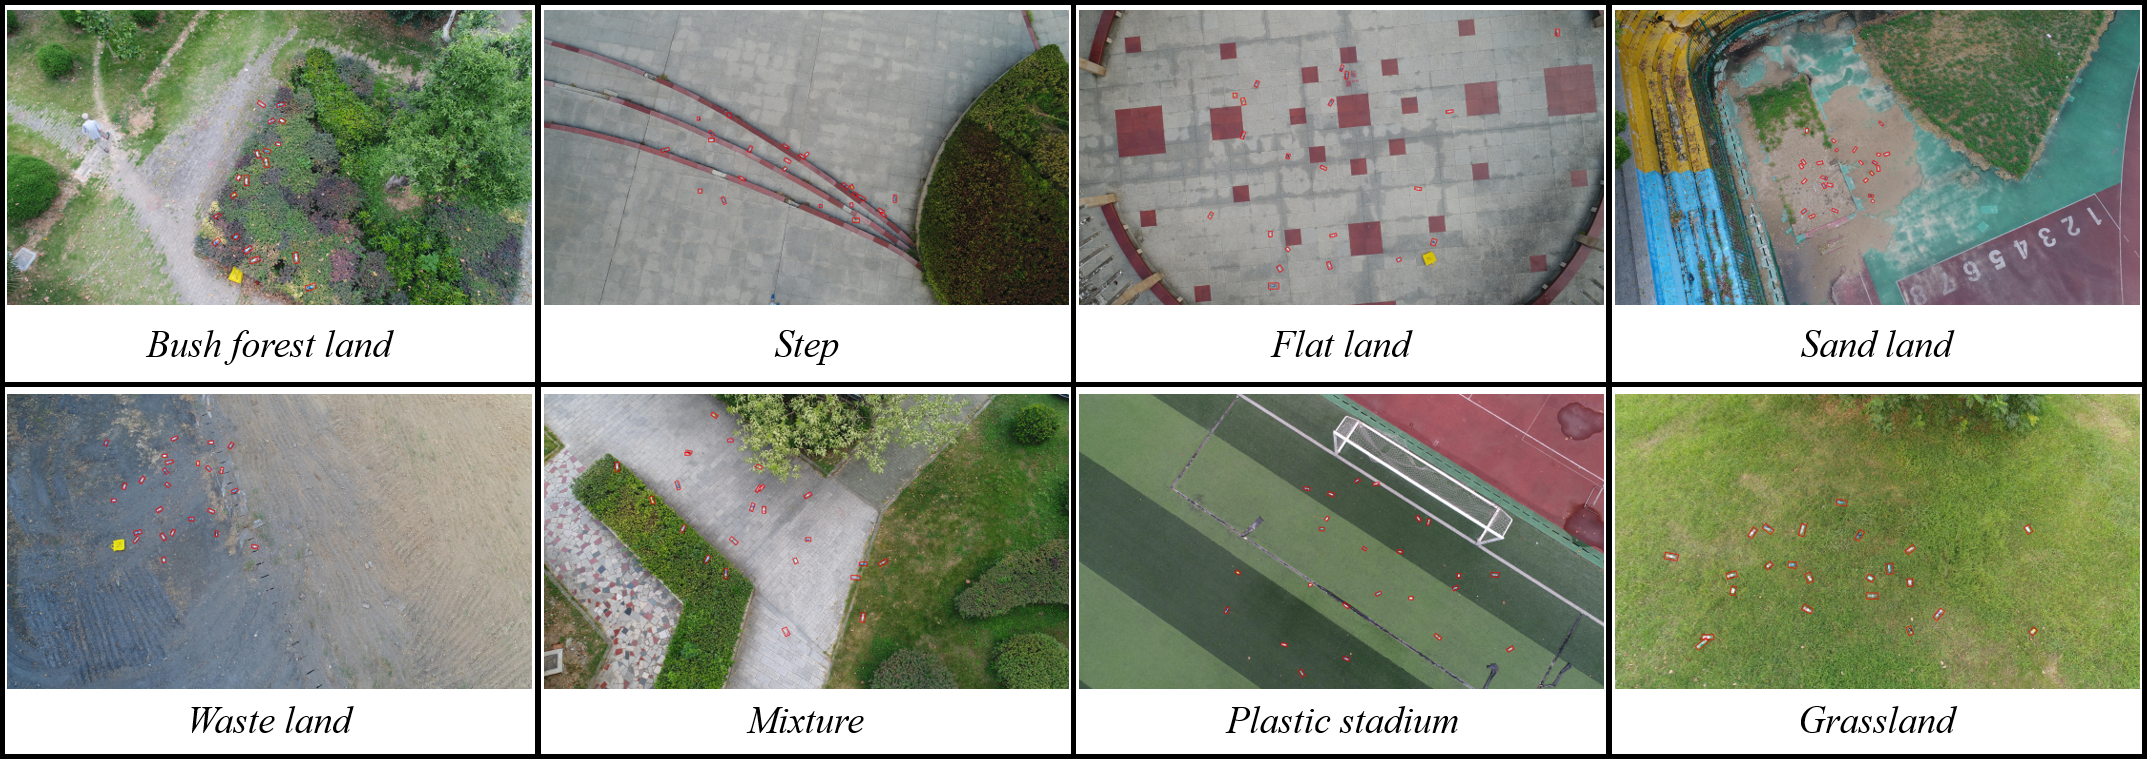
\includegraphics[width=\linewidth]{images/UAV-BD1.png}
	\caption{Samples of annotated images in UAV-BD. We show one full image which size is $ 5472\times 3078 $ per each scene.}
	\label{fig:dataset-original-image}
\end{figure}



\begin{figure}
	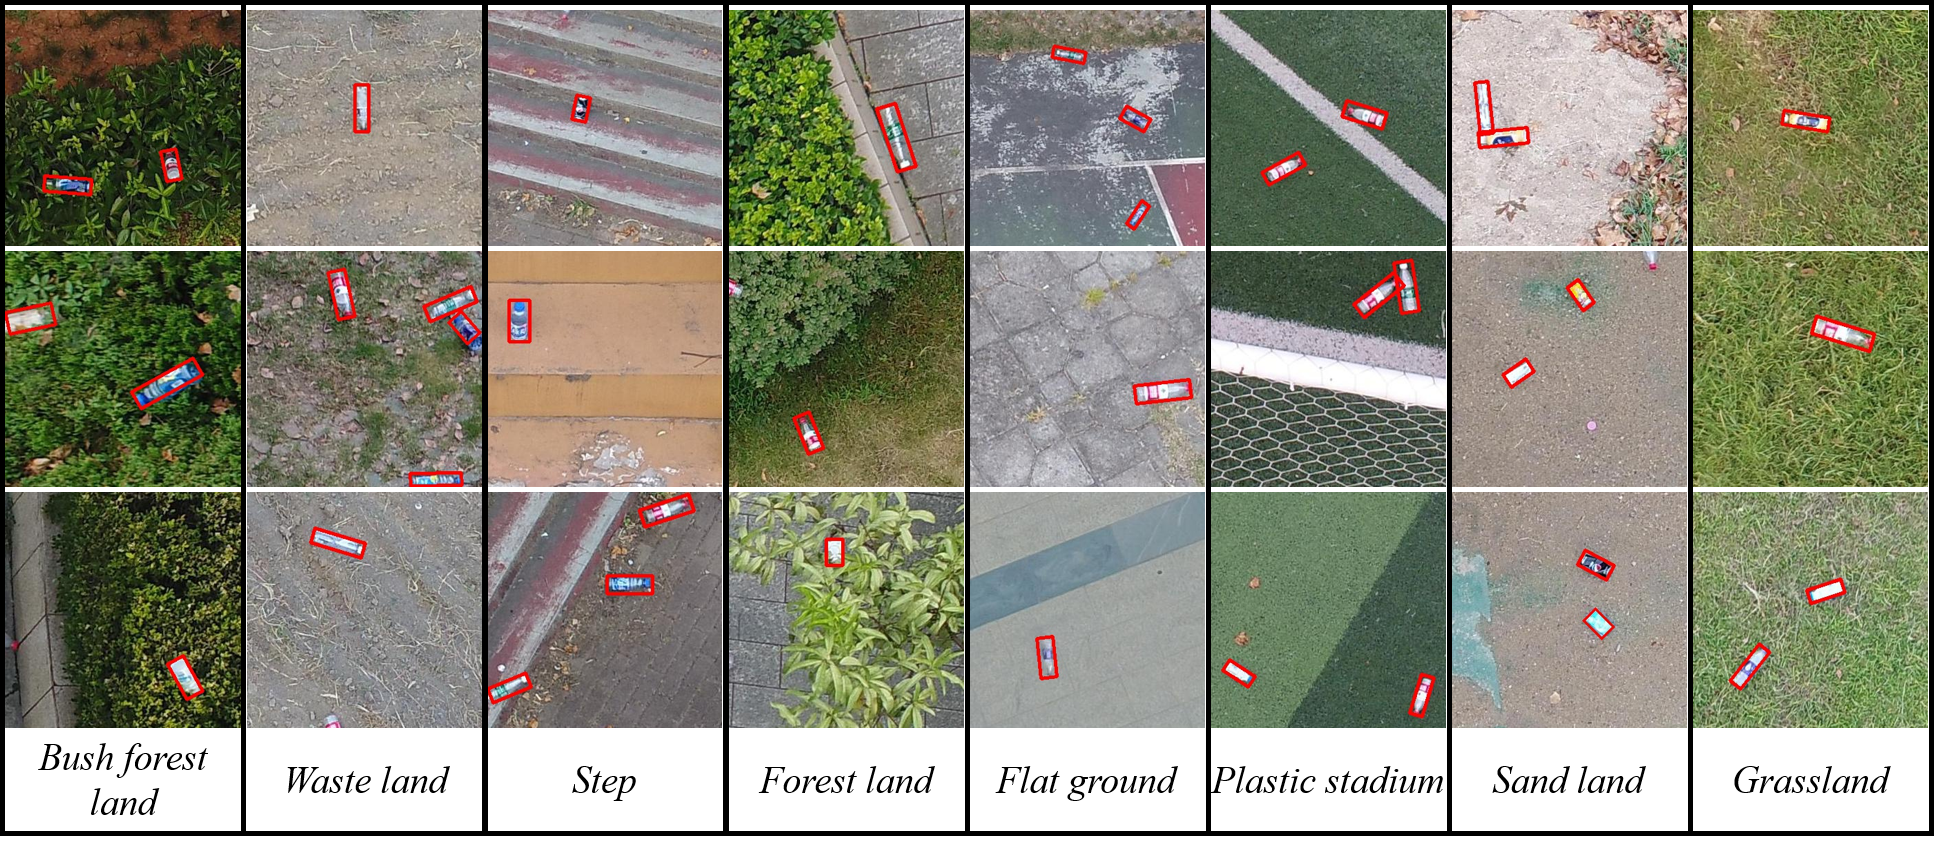
\includegraphics[width=\linewidth]{images/UAV-BD2.png}
	\caption{Sample of annotated images in UAV-BD. We show three images which sizes are $ 342\times 342 $ per each scene.}
	\label{fig:dataset-cut-image}
\end{figure}



%% 2. 数据标注方式
\subsection{Annotation method}
\label{ssec:annotation_method}




We build the UAV-BD for the bottle detection problem by collecting bottle images using UAV. In the annotating stage, we consider different ways to annotate images. In computer vision field, many visual concepts such as region descriptions, objects, attributes, and relationships, are annotated with horizontal bounding boxes, as show in \cite{DOTA, boundingbox}. A common description of horizontal bounding boxes is $(c_x, c_y, w, h)$ or $ (x, y, w, h) $, where $(c_x, c_y)$ is the center location of horizontal bounding box, $w, h$ are the width and height of the horizontal bounding box, $ (x, y) $ is the top left location of the horizontal bounding box, respectively\cite{DOTA}. 

Objects without many orientations can be adequately annotated with this method. However, bounding boxes annotated in this way cannot accurately or compactly outline oriented instances such as objects in UAV images. In UAV images, the overlap between two bounding boxes is sometimes very large that state-of-the-art object detection methods cannot diffetentiate them\cite{DOTA}. At the same time, horizontal bounding box may contain lots of backgrounds while annotating the target, it's especially the kind of objects with large aspect ratios. In order to remedy these, we need to find an annotation method suitable for oriented bottles in UAV images.

An option for annotating oriented objects is arbitrary quadrilatral bounding boxes, this annotation method can be denoted as ${(x_i, y_i), i=1,2,3,4}$, where $(x_i, y_i)$ denotes the positions of the oriented bounding boxes' vertices in the image\cite{DOTA}. The vertices are arranged in a clockwise order. But due to bottles are rigid, almost no deformation, so we choose other way which is $\theta$-based oriented bounding box which is adopted in some text detection benchmarks, namely $(c_x, c_y, w, h, \theta)$, where $\theta$ denotes the angle from the horizontal direction of the horizontal bounding box\cite{DOTA}. The tool for annotating is roLabelImg\footnote{\url{https://github.com/cgvict/roLabelImg.git}}.

\begin{figure}
	\centering
	\subfigure[Normal annotation method]
	{
		\label{angle}
		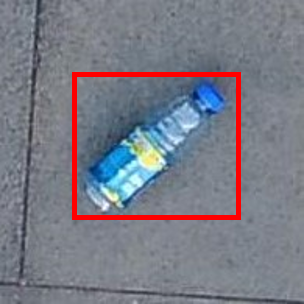
\includegraphics[width=0.45\linewidth]{images/bottle_advantage_2.png}
	}
	\subfigure[Our annotation method]
	{
		\label{size}
		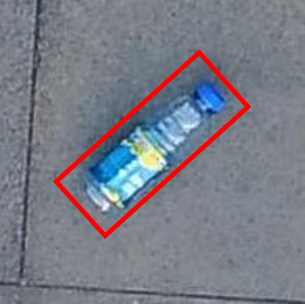
\includegraphics[width=0.45\linewidth]{images/bottle_advantage_1.png}
	}
	\caption{Comparison of traditional bounding box and rotatable bounding box. }
\end{figure}



\subsection{Dataset Splits}

In order to ensure that the training and testing data distributions approximately match, we randomly select $ 64\% $ of the UAV-BD as the training data, $ 16\% $ as validation data, and $ 20\% $ as the testing data. We will publicly provide all the full images and segmented images with ground truth for UAV-BD.



%% 3. 数据量统计 
\subsection{Dataset Statistics}
\label{ssec:Dataset_Statistics}
UAV images are usually very large in size compared to conventional images datasets. The size of full images in UAV-BD is $ 5472\times 3078 $ while most images in conventional datasets (e.g. PASCAL VOC and Microsoft COCO) are no more than $ 1000 \time 1000 $\cite{RCNNforSmall}. We firstly make annotations on the full images without segmenting it into pieces to avoid the single instances is segmented into different pieces. But we find full image is too large to be trianed CNN based algorithms. So we segment full images into $ 144 $ small pieces, the size of piece is $ 342\times 342 $, note that we abandon the instances at the border. We will use small pieces to train CNN based detection model. 


The statistics of the UAV-BD is shown in the Table\ref{statistics}, where $ n_1 $ is the full images number for each scene, $ n_2 $ is the small images number for each scene, $ n_3 $ is the number of instances in full images for each scene, $ n_4 $ is the number of instances in small images for each scene. So UAV-BD contains about $ 34,791 $ object instances in $ 25,407 $ images. The "Grassland" scene has the largest number of object instance: $ 7,795 $ instances in $ 5,785 $ images. The "Step" scene has the smallest number of instances: $ 2106 $ instances in $ 1,325 $ images.



% Please add the following required packages to your document preamble:
% \usepackage{booktabs}
\begin{table}
	\centering
	\small
	\caption{Images and instances number in UAV-BD}
	\label{statistics}
	\begin{tabular}{@{}ccc|cc@{}}
		\toprule
		Scenes     & $n_1$& $n_2$ & $n_3$ & $n_4$  \\ \midrule
		Bush forest land       & 230  & 4134  & 1812  & 3047  \\
		Waste land     & 379  & 7598  & 4355  & 5800  \\
		Step       & 135  & 2691  & 1325  & 2106  \\
		Forest land    & 285  & 5724  & 3702  & 4891  \\
		Flat land       & 134  & 2803  & 1538  & 2142  \\
		Plastic stadium & 336  & 6807  & 4180  & 4998  \\
		Sand land       & 249  & 5570  & 2704  & 4008  \\
		Grassland       & 456  & 9029  & 5778  & 7787  \\ \midrule
		Total      & 2204 & 44356 & 25394 & 34779 \\ \bottomrule
	\end{tabular}
\end{table}


Bottles are usually rigid body, so we can get some prior information for training out detection model, for example, we can use angle distribution, size distribution, ratio distribution, etc. to improve the performance of detection model. For UVA-BD, we plot angle, size and ratio distribution which are illustrated in Fig.\ref{distribution}. We can see that bottles' angle in images are almost uniform in Fig.\ref{angle}. Bottles' size are usually range from $500\text{pixel}^2 $ to $3000\text{pixel}^2 $. Bottles' ratio are usually range from $ 1.0 $ to $ 4.0 $. Note that we use these statistics data to design detection models.


\begin{figure}
	\centering
	\subfigure[angle distribution]
	{
		\label{angle}
		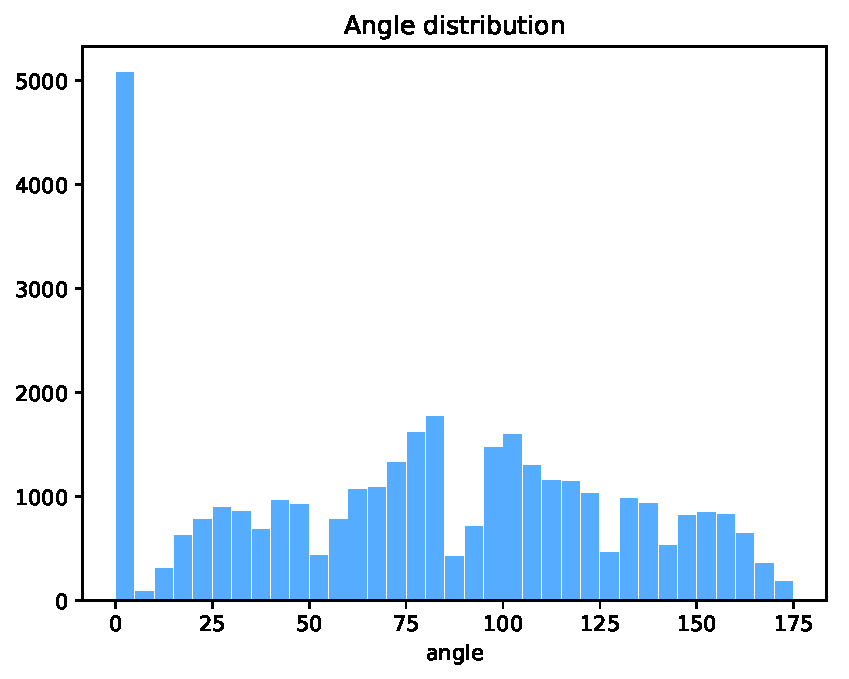
\includegraphics[width=0.45\linewidth]{images/angle_hist.pdf}
	}
	\subfigure[size distribution]
	{
		\label{size}
		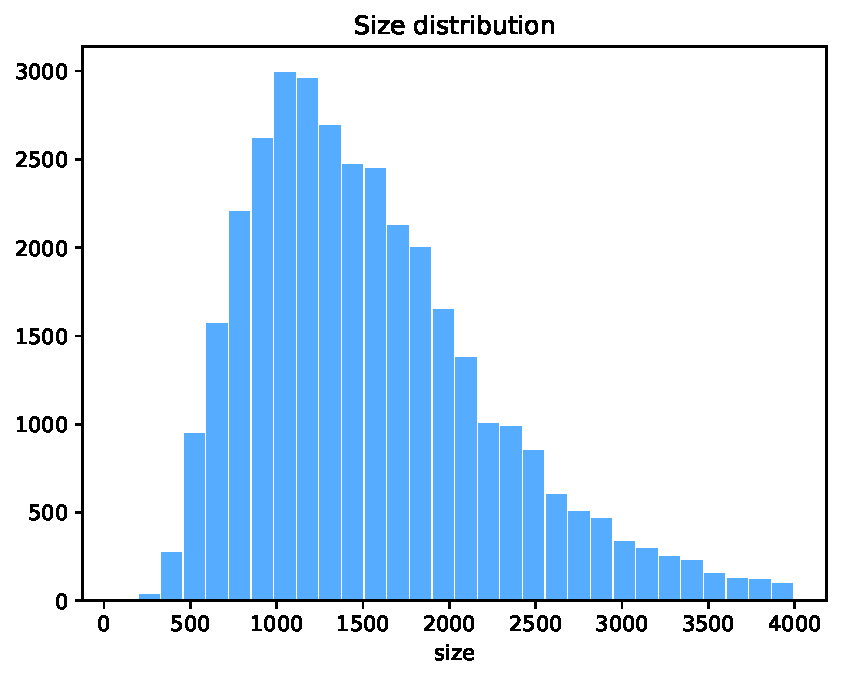
\includegraphics[width=0.45\linewidth]{images/size_hist.pdf}
	}
	\subfigure[ratio distribution]
	{
		\label{size}
		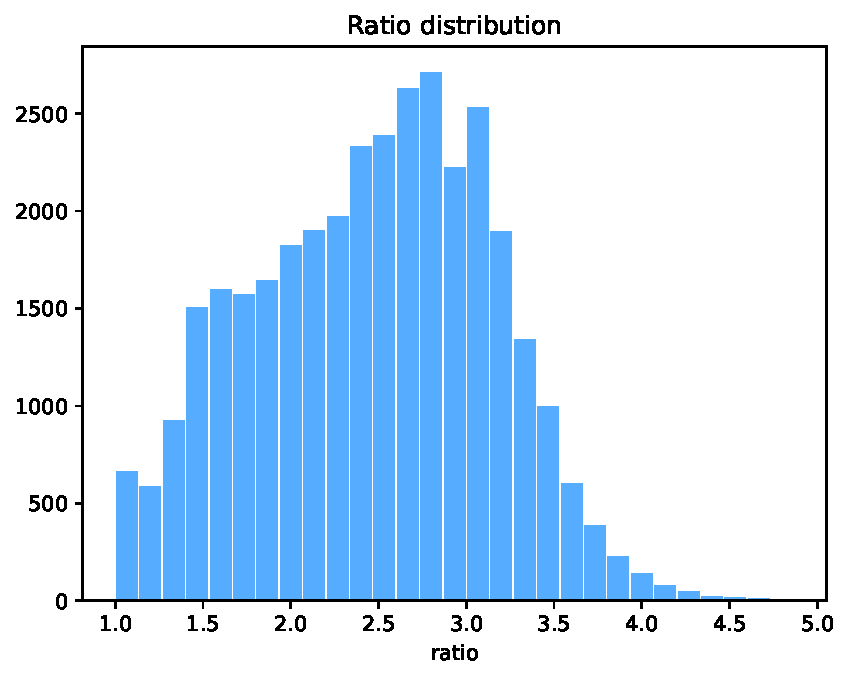
\includegraphics[width=0.45\linewidth]{images/ratio_hist.pdf}
	}
	\caption{The angle, size and ratio distribution of UAV-BD}
	\label{distribution}
\end{figure}




\section{Baselines and Methods}
\label{sec:exp}

%% 1. 简要再次介绍数据集

All experiments are performed using UAV-BD, the training, validation and testing date include $ 16258 $, $ 4065 $ and $ 5081 $ images, respectively. Note that the images for training, testing and validation are the size of $ 342 \time 342 $. The whole UAV-BD contains $ 16258 $ images with $ 22211 $ instances for training, $ 5081 $ images with $ 6944 $ instances for testing and $ 4055 $ images with $ 5624 $ instances for validation.

%% 2. 实验使用了 4 中基于深度学习的方法

Here, we present three different approaches to our task, which vary by their use of detection framework and data annotating method. For horizontal object detection, we select Faster R-CNN\cite{FasterRCNN} and SSD\cite{SSD} as our baseline testing algorithms for their excellent performance on general object detection. For oriented object detection, wo modify the original Rotation Region Proposal Networks(RRPN) algorithm\cite{RRPN} such that it can predict properly oriented bounding boxes denoted as $ \{c_x, c_y, w, h, \theta\} $. Note that ($ c_x $, $ c_y $) is the central coordinate of the oriented bounding box, $ w $ and $ h $ is the width and height of the oriented bounding box, $ \theta $ is the rotation angle of the oriented bounding box.

%\begin{itemize}
%	
%	\item \textbf{Faster R-CNN}
%	
%	\item \textbf{SSD}
%	
%	\item \textbf{RRPN}
%	
%	\item \textbf{DRBox}
%\end{itemize}


\subsection{Baselines with Horizontal Bounding Boxes}

Ground truths for horizontal bounding boxes(HBB) experiments are generated by calculating the axis-aligned bounding boxes over original bounding boxes. To make it fair, we keep all the experiments' setting and hyper-parameters the same as depicted in corresponding papers\cite{FasterRCNN, SSD, YOLOv2}.

The experimental results of HBB prediction are shown in Fig.\ref{fig:result}. In Fig.\ref{fig:result}, first row illustrates the results for Faster R-CNN, second row illustrates the results for SSD, third row illustrates the results for YOLOv2.


\begin{figure}
	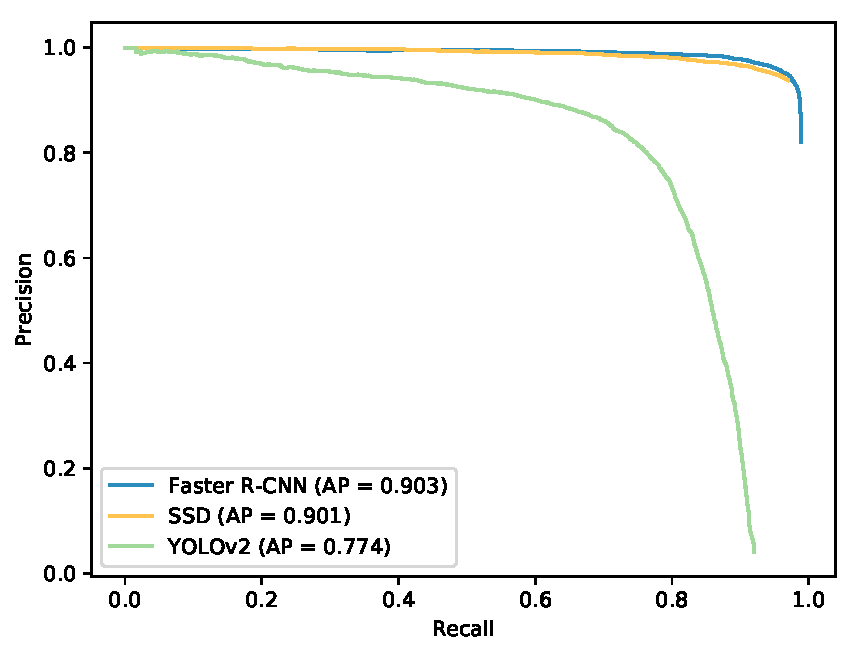
\includegraphics[width=\linewidth]{images/pr_bbox.pdf}
	\caption{Numerical results (AP) of baseline models evaluated with HBB ground truths.}
	\label{fig:pr_bbox}
\end{figure}

\subsection{Baseline with Oriented Bounding Boxes}

Prediction of oriented bounding boxes(OBB) is difficult because the state-of-the-art detection methods are not designed for oriented objects. Therefor, we choose Rotation Region Proposal Networks(RRPN)\cite{RRPN} as the framework for its accuracy and efficiency, then we modify it to adapt UAV-BD on the basis of dataset statistics in section \ref{ssec:Dataset_Statistics}.

For RRPN, it's based on Faster R-CNN, in Faster R-CNN, Region of Interests(RoIs) generated by Region Proposal Network(RPN) are rectangles which can be write as $ R = (x_{min}, y_{min}, x_{max}, y_{max}) = (c_x, c_y, w, h) $. These RoIs have regressed from $ k $ anchors which are generated by some predefined scales and aspect ratios. But in RRPN, it uses predefined scales, aspect ratios and \textit{angles} to generate RoI, so RRPN can predict oriented bounding boxes which can be written as $ R=(c_x, c_y, w, h, \theta) $. In the section \ref{ssec:Dataset_Statistics}, we analyzed the size, aspect ratio and angle distributions of UAV-BD, so we can select reasonable scales, aspect ratios and angles value to generate new anchors which are shown in Fig.\ref{fig:anchors}. 

The experimental results of RRPN prediction are shown in Fig.\ref{fig:result}. In Fig.\ref{fig:result}, forth row illustrates the results for RRPN.



\begin{figure}
	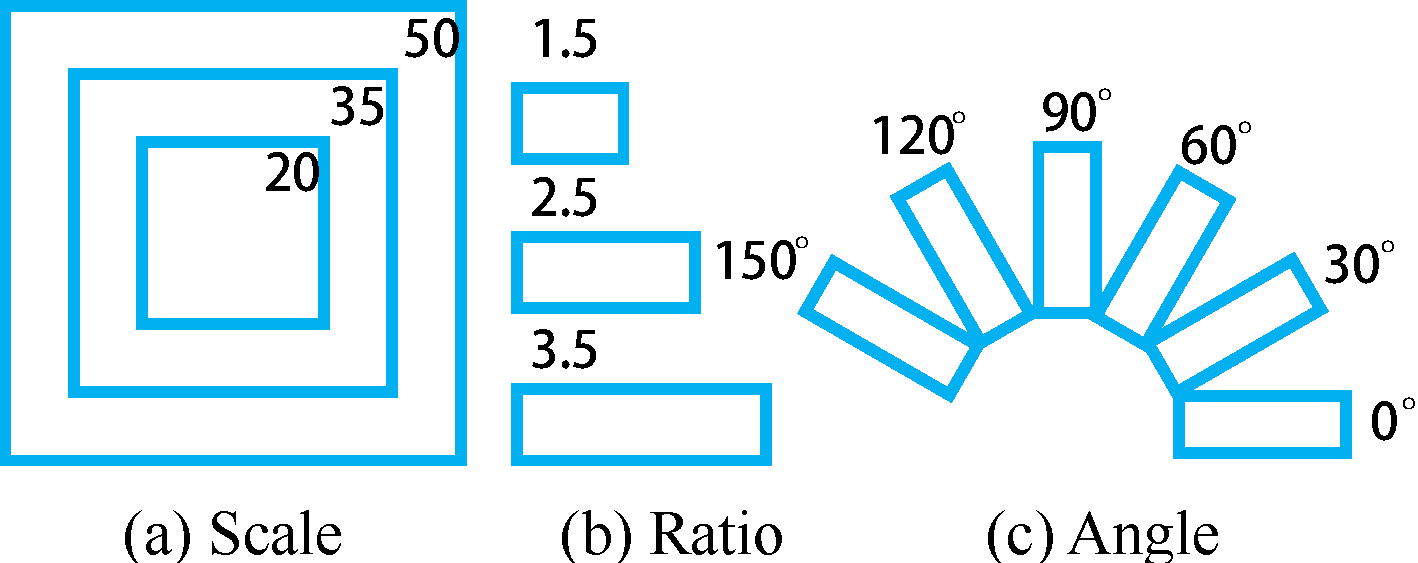
\includegraphics[width=\linewidth]{images/scale_ratio_angle.pdf}
	\caption{Anchor strategy in our framework of RRPN}
	\label{fig:anchors}
\end{figure}

\begin{figure}
	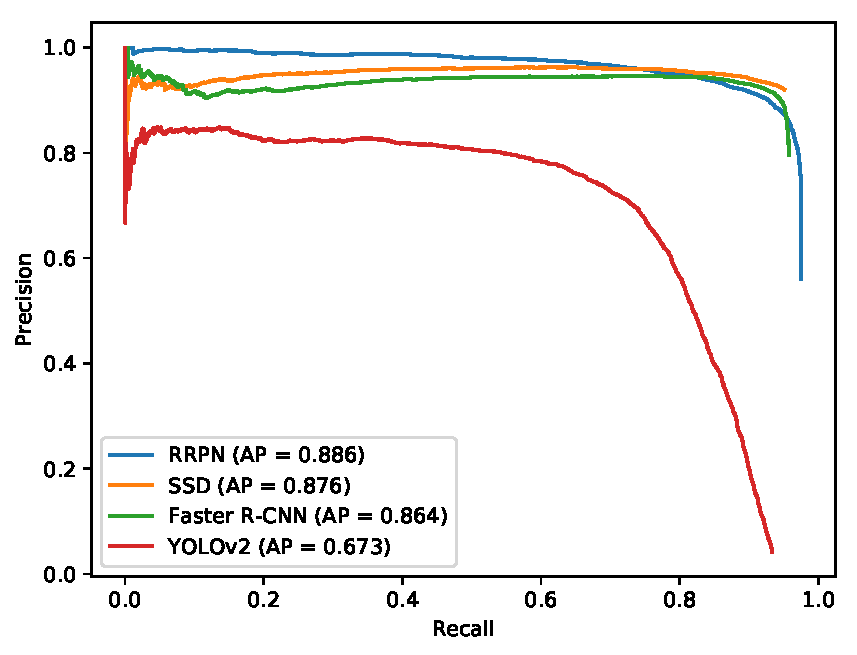
\includegraphics[width=\linewidth]{images/pr_rbbox.pdf}
	\caption{Numerical results (AP) of baseline models evaluated with OBB ground truths.}
	\label{fig:pr_rbbox}
\end{figure}

%\begin{figure}
%	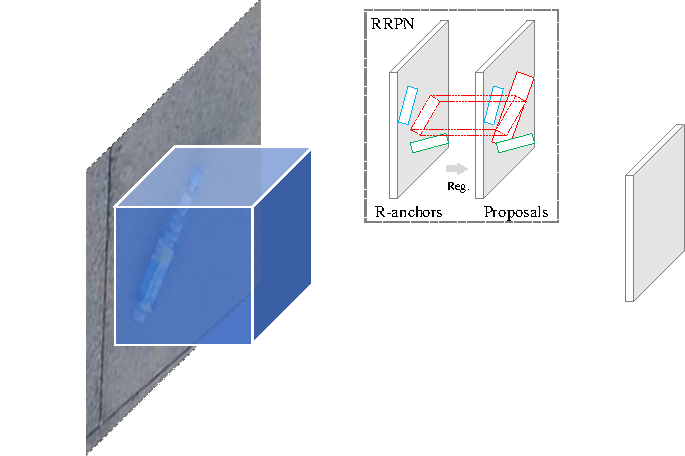
\includegraphics[width=\linewidth]{images/RRPN.pdf}
%	\caption{Rotation based text detection pipline}
%	\label{fig:pipline}
%\end{figure}


\subsection{Experimental Analysis}

Fig.\ref{fig:pr_bbox} show the quantitative comparison result of three baseline models evaluated with HBB ground truth, measured by precision-recall curve and AP values. For evaluation metrics, we adopt the same AP calculation as for PASCAL VOC. As can be seen from it, Faster R-CNN, SSD, YOLOv2 obtain $ 90.3\% $, $ 90.1\% $, $ 77.4\% $ performances, respectively.


Fig.\ref{fig:pr_rbbox} show the quantitative comparison result of five baseline methods evaluated with OBB ground truth, measured by precision-recall curve and AP values. As can be seen from it, RRPN, SSD, Faster R-CNN, YOLOv2, DRBox obtain $ 88.6\% $, $ 87.6\% $, $ 86.4\% $, $ 67.3\% $, $ 32.7\% $ performances, respectively.

In Fig.\ref{fig:result}, we compare the results between objects detection experiments of HBB and OBB. For oriented objects shown in Fig.\ref{fig:result}, location precision of objects in HBB 
experiments are much lower than OBB experiments and results are suppressed through progress operations. So OBB regression is the correct way for oriented object detection that can be really integrated to real applications.


\begin{figure}
	\includegraphics[width=\linewidth]{images/result.png}
	\caption{Visualization results of testing on UAV-BD using well-trained Faster R-CNN, SSD and RRPN. \textbf{TOP} to \textbf{Bottom} respectively illustrate the results for Faster R-CNN, SSD, YOLOv2 and RRPN.}
	\label{fig:result}
\end{figure}










%\begin{figure}
%	\centering
%	\subfigure[angle distribution]
%	{
%		\label{angle}
%		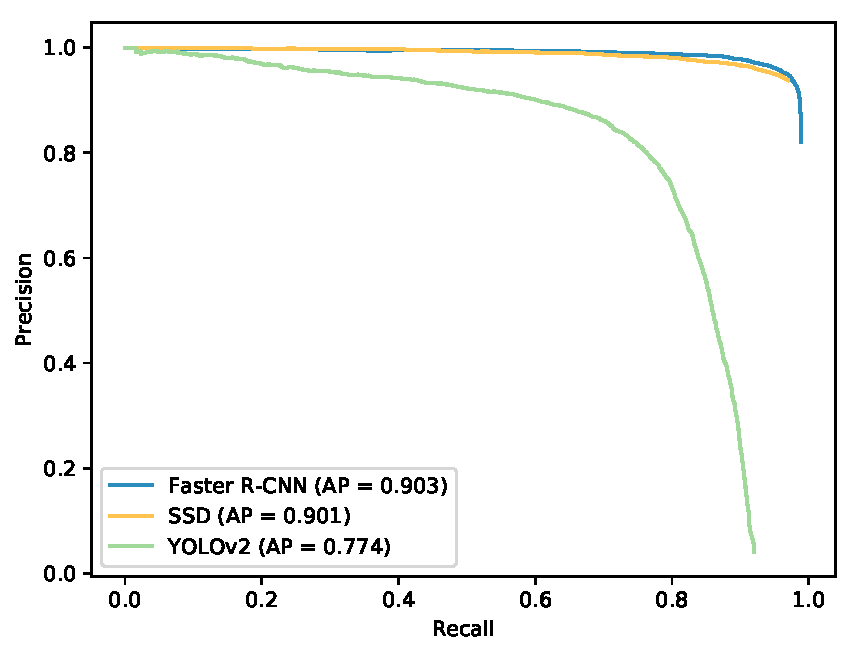
\includegraphics[width=0.45\linewidth]{images/pr_bbox.pdf}
%	}
%	\subfigure[size distribution]
%	{
%		\label{size}
%		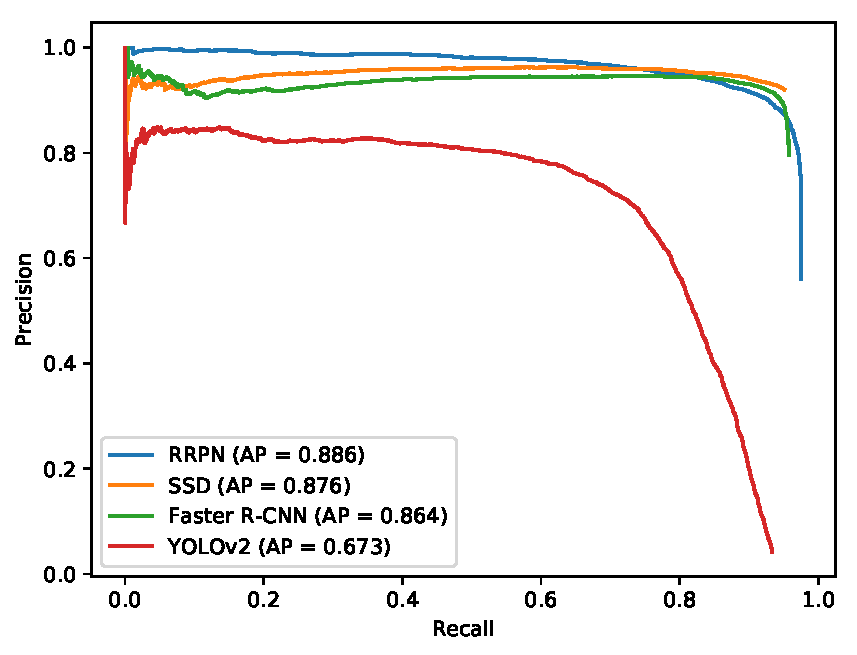
\includegraphics[width=0.45\linewidth]{images/pr_rbbox.pdf}
%	}
%	\caption{The precision-recall curve for bottle detection for Faster R-CNN, SSD and RRPN}
%	\label{fig:PR}
%\end{figure}





%\renewcommand{\algorithmicrequire}{\textbf{Input:}}
%\renewcommand{\algorithmicensure}{\textbf{Output:}}


%\begin{algorithm}
%	\caption{IoU computation}
%	\begin{algorithmic}[1]
%		\Require Rectangle $ R_1, R_2,\cdots,R_N $
%		\State IoU[1, $ N $][1, $ N $] $ \gets $ 0
%		\For {each pair of $ R_i, R_j(i<j) $} 
%		\State Point set $ PSet \gets \emptyset $
%		\State Add intersection points of $ R_i $ and $ R_j $ to $ PSet $
%		\State Add the vertices of $ R_i $ inside $ R_j $ into $ PSet $
%		\State $ \text{IoU}(i,j) \gets (\text{Area}(R_i) + \text{Area}(R_j) - I)/I $
%		\EndFor
%		\Ensure IoU
%	\end{algorithmic}
%\end{algorithm}



\section{Conclusion and Future Work}
\label{sec:conclusion}


In this paper, we have built a large-scale dataset for bottle detection in UAV images, i.e., UAV-BD. In contrast to general object detection benchmarks, we annotate a huge number of well-distributed bottles with oriented bounding boxes. We believe this dataset is challenging and very useful for real vision based bottle recycling. Based on this dataset, we also establish a benchmark for bottle detection and show the feasibility to produce oriented bounding boxes which provides more useful information for bottle grasping.

In future work, we will focus on locating and recycling bottles in the real-world using UAV.





\section*{Acknowledgment}

We thanks Ruixiang Zhang, Jiaqi Xiong, Siyao Zhou, Hao Li, and all the others who involoved in the annotations of UAV-BD.

%\section*{References}

\bibliographystyle{IEEEtran}
\bibliography{paper}




%\begin{thebibliography}{00}
%\bibitem{b1} G. Eason, B. Noble, and I. N. Sneddon, ``On certain integrals of Lipschitz-Hankel type involving products of Bessel functions,'' Phil. Trans. Roy. Soc. London, vol. A247, pp. 529--551, April 1955.
%\bibitem{b2} J. Clerk Maxwell, A Treatise on Electricity and Magnetism, 3rd ed., vol. 2. Oxford: Clarendon, 1892, pp.68--73.
%\bibitem{b3} I. S. Jacobs and C. P. Bean, ``Fine particles, thin films and exchange anisotropy,'' in Magnetism, vol. III, G. T. Rado and H. Suhl, Eds. New York: Academic, 1963, pp. 271--350.
%\bibitem{b4} K. Elissa, ``Title of paper if known,'' unpublished.
%\bibitem{b5} R. Nicole, ``Title of paper with only first word capitalized,'' J. Name Stand. Abbrev., in press.
%\bibitem{b6} Y. Yorozu, M. Hirano, K. Oka, and Y. Tagawa, ``Electron spectroscopy studies on magneto-optical media and plastic substrate interface,'' IEEE Transl. J. Magn. Japan, vol. 2, pp. 740--741, August 1987 [Digests 9th Annual Conf. Magnetics Japan, p. 301, 1982].
%\bibitem{b7} M. Young, The Technical Writer's Handbook. Mill Valley, CA: University Science, 1989.
%\end{thebibliography}

\end{document}
